
\chapter{Analysis and Theoretical Foundation}
\label{ch:analysis}

%Together with the next chapter takes about 60\% of the whole paper
%
%The purpose of this chapter is to explain the operating principles of the implemented application.
%Here you write about your solution from a theory standpoint - i.e. you explain it and you demonstrate its theoretical properties/value, e.g.:
%\begin{itemize}
% \item used or proposed algorithms
% \item used protocols
% \item abstract models
% \item logic explanations/arguments concerning the chosen solution
% \item logic and functional structure of the application, etc.
%\end{itemize}
%
%{\color{red} YOU DO NOT write about implementation.
%
%YOU DO NOT copy/paste info on technologies from various sources and others alike, which do not pertain to your project.
%}

\section{Overview}
\label{sec:analysis-overview}
The project consists of several geographically-distributed components communicating \
to each other.
Since we are talking about a remote-controlled robot, it is obvious that 2 \
of these components are the robot and the control interface.
An important factor in determining what the other components are is the \
type of communication between the robot and the control interface (how the \
robot will transmit the video and how the controller will transmit the \
commands): Peer-to-peer or client-server.

In a client-server architecture, both the controller and the robot are connected \
to a server, and the server is in charge of relaying control commands from controller \
to the robot, and of processing robot images and transmitting them further to the \
controller.
In this architecture, image processing is only done once server-side, after which \
the result can be sent to multiple clients.
However, the server must make sure  only one controller client can send control \
messages to the robot.
This entails two more components: an image processor (that is in charge of processing \
robot images) and one server that is in charge of sending robot images to clients and \
of sending client commands to the robot.

The other type of architecture is Peer-to-peer.
In this case, the robot sends the video directly to the controllers, thus eliminating \
some communication overhead.
However, this introduces a new issue related to image processing.
If the image processing is done on the robot, then the robot will most likely require \
a GPU in order to speed up the processing and allow real-time video transmission.
However, this leads to a higher energy consumption, lower autonomy and increased costs.
On the other hand, if the image processing is done on the machine on which the controller \
runs, then that machine will require a powerful GPU, which contradicts our usability \
requirements, which states that the users controlling the robot should be able to use any \
screen, no matter the hardware (to a certain degree).
Additionally, the robot should be aware of all controllers so that it knows where \
to transmit the images, which introduces more coupling between the robot and \
controller.

Having considered the arguments above, I decided to go with the client-server \
architecture.
Besides the fact that it allows running object detection on specialized hardware \
without impacting the drone autonomy or requiring state-of-the-art GPU for controllers,\
it also decouples the drone from controllers.

\begin{figure}[ht]
    \label{fig:high-level-arch}
    %\centering
    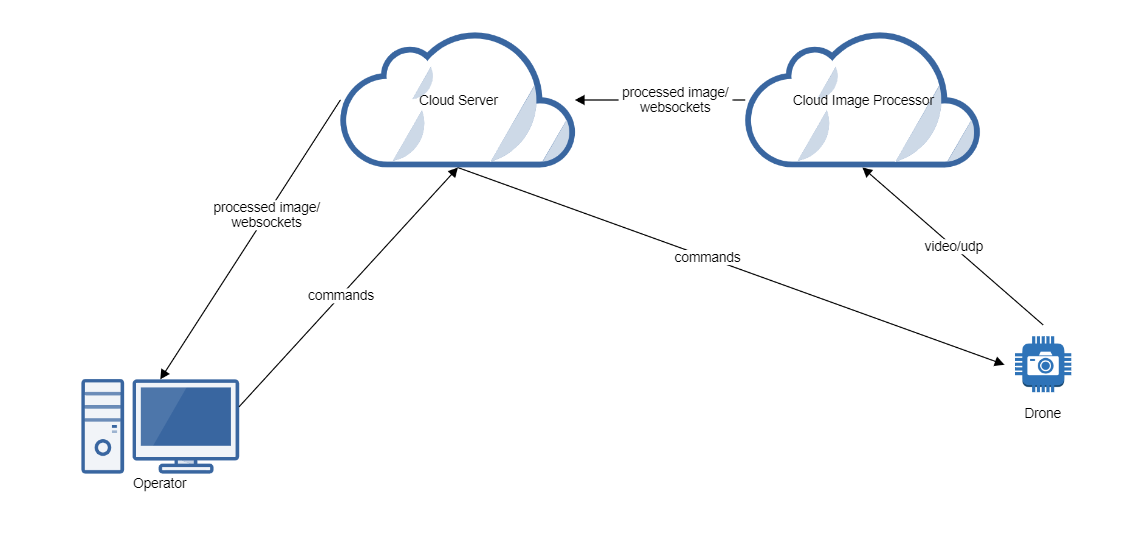
\includegraphics[width=15cm, height=50cm,keepaspectratio]{img/overview.png}
    \caption{High Level Architecture}
\end{figure}

Once I decided upon the architecture, I had to decide what type of \
client I would implement.
There were three possible options:
\begin{enumerate}
    \item Desktop client
    \item Mobile client
    \item Browser client
\end{enumerate}

After carefully considering all three options, I decided to implement \
a browser client for the following reasons:
\begin{enumerate}
    \item \textbf{Cross-platform support} Browser clients run on all \
            modern browsers on all desktop and mobile platforms.
            A Desktop application would have to have at least  3 \
            distributions (Linux, Windows, MacOS), while a mobile \
            platform would need to have at least 2 distributions
            (IOS and Android)
    \item \textbf{Application Update} Since the web client's source \
            reside on the server and are downloaded every time a user \
            runs the application, I have full control over what \
            version runs on the users' machines and don't have to \
            rely on them to update their applications nor do I have to maintain \
            deprecated APIs in production so that older versions of \
            clients can still run.
    \item \textbf{Versatility} There is a possibility that future \
            requirements might be incompatible \
            with a browser application.
            With that in mind, there are open-source technologies \
            that can turn browser applications \
            into native desktop or native mobile applications.
\end{enumerate}

\section{Communication Protocols}
\label{sec:analysis-comms-protocols}
As seen in the diagram ~\ref{fig:high-level-arch},
every image is transmitted twice: once from drone to the server, and once from \
the server to the controller.
Ideally, in order to reduce latency, we would use UDP sockets for both transmissions.
However, since the controller should work in a browser, the connection between the controller \
and the server should be TCP.
As for the transmission between robot and the server, we are free to use UDP sockets, \
even if this means some packets could be dropped.
However, since the transmission will be done on Google premium quality networks, \
packet loss is expected to be low to zero.
As a result, the transmission between server and controller is expected to be slower \
than the transmission between robot and server (since TCP sockets require several round-trips \
in order to validate the content and possibly retransmit packets).
In order to minimize the effects of the TCP connections, the server should be \
geographically located as close as possible to the controller.
The closest datacenters to Romania are in Frankfurt and Milan for Amazon and in \
Frankfurt and Zurich for Google, with a Warsaw datacenter in construction.

As for the drone commands, these cannot be lost, so they will be transmitted using \
TCP sockets.
The most efficient TCP method of communication between a browser based \
application and a server is using websockets, which will be presented \
below.

\subsection{Websockets}
\label{subsec:analysis-websockets}
According to ~\cite{TeamTreeHouseWebSockets}, websockets appeared \
due to the need to establish efficient bi-directional connections \
between browser applications and servers.
After 2005, when AJAX appeared, which allowed browser applications \
to query a server for data without reloading the web page, \
developers became more interested in establishing bi-directional \
communication between client and server.
The first method was using long-polling.
As defined by ~\cite{WikiLongPolling}, long polling is a technique \
in which the client executes a normal connection, but expects that \
the server could not respond in a short while.
The server keeps the connection open up until it has new information \
that it can transmit as an HTTP/S response.
Then the client closes the existing HTTP/S request and makes a \
new one.
The downside of long polling is that both the initial HTTP/S \
request and the response contain a lot of specific HTTP headers \
and cookies, most or all of which are useless.
This introduces a considerable latency, especially when the number \
of concurrent connection grows.

Websockets appeared as a way to minimize latency, allowing true \
bi-directional communication.
Websockets are initialized with an HTTP request to the server, \
though there are a few differences.
The http/s scheme is replaced with a ws/s scheme specific to \
websockets.
Additionally, the request also contains an \textit{Upgrade} \
headers with the value \textit{websocket}

\begin{verbatim}
GET ws://localhost:8080/ HTTP/1.1
Origin: http://localhost:8080
Connection: Upgrade
Host: localhost:8080
Upgrade: websocket
\end{verbatim}

If the server has support for websockets, it sends back a response \
that also contains the \textit{Upgrade} header.

\begin{verbatim}
HTTP/1.1 101 WebSocket Protocol Handshake
Date: Wed, 17 Jun 2020 10:07:34 GMT
Connection: Upgrade
Upgrade: WebSocket
\end{verbatim}

After this handshake completes, the server and client replace the \
HTTP connection with a websocket connection which uses the same \
TCP/IP connection.
Then both the server and the client can send data to each other \
in a truly bi-directional communication.
The data is transmitted as websockets messages, each message \
consisting of multiple frames.
Only after all the frames have been received can the receiver \
begin to process the data.

Even though messages still require an additional 4\-12 frames \
of data in order for them to be routed correctly, the \
overhead is still considerably smaller than the overhead for \
normal HTTP requests, and the latency is reduced considerably.


\section{Algorithms}
\label{sec:analysis-algorithms}

\subsection{Object detection}
\label{subsec:analysis-object-detection}

For object detection I have chosen to use deep neural networks due to their \
increased performance (speed and accuracy) compared to other ML-based algorithms.\
More specifically, I decided to use the  MobileNetV2~\cite{mobilenet2} neural \
network with SSD (single shot detection).
MobileNet works as a feature extractor, with the output of its last layers \
connected to the input of the SSD network.

In order for deep neural networks to be effective, they need to be trained on \
large datasets.
Some common such datasets are:
\begin{itemize}
    \item the Microsoft COCO dataset ~\cite{COCO} (about 300k images, out of \
            which more than 200k are labeled)
    \item the KITTI dataset ~\cite{kitti}
    \item Open Images dataset ~\cite{openimages} (over 1.7 million images)
\end{itemize}

A neural network takes a considerable amount of time to train on such datasets \
even with state-of-the-art hardware.
For this reason, there are a number of pre-trained models available on the \
internet.
\footnote{https://github.com/tensorflow/models/blob/master/research/object\_detection/g3doc/detection\_model\_zoo.md} \
contains a list of pre-trained models that could be used for object detection.
The most efficient, taking into consideration both accuracy and execution \
speed, seems to be \textbf{ssdlite\_mobilenet\_v2\_coco}, which is why I \
chose to use it the drone.

\subsection{Object Tracking}
\label{subsec:analysis-object-tracking}
I also considered using tracking algorithms in conjunction \
with detection algorithms.
However, after careful analysis, I decided that the performance \
impact brought by the tracking algorithms would be too great \
compared to the business value.
On the one hand, detection algorithms should be run every frame \
in order to detect possible new objects.
If I applied tracking algorithms as well, in most cases the \
bounding boxes generated by the tracker and by the detector \
would overlap or share \~80\% surface, in which case the most \
likely case would be that the tracking algorithm would need \
correction.


\section{Robot}
\label{sec:analysis-robot-control}
In order to meet all functional requirements, the robot must consist of \
a central processing unit, a chassis, 4 dc motors and wheels, a motor shield, \
a camera and a 4G adapter, as shown in figure ~\ref{fig:robot-scheme}.

\begin{figure}[ht]
    \label{fig:robot-scheme}
    %\centering
    \includegraphics[keepaspectratio]{img/land-drone-bb4.png}
    \caption{Robot Scheme}
\end{figure}

The software components running on the robot are the engine control and the \
I/O control (handling all outside communication and the camera itself for \
performance reasons).
In order to enforce low couping between these components and other components \
that could be added in the future, they are deployed separately and run in \
different processes.
The only means of communication is a queue, more specifically a RabbitMQ that \
runs on the robot.
The queue is used in order to transmit commands from the I/O control to the \
engine control for now.
This decoupled architecture prevents changes in a component from affecting \
other components and allows independently deploying several components, thus \
increasing extendability.


\subsection{Image transmission}
\label{subsec:analysis-image-transmission}
 I needed to devise an algorithm that would allow to one source to send images to several receivers that are
 not on the same network and at considerable distances, and at the same time having a delay as small as possible.
 Since the sender and the receivers won't be on the same network, they will need to interact via a 3rd component,
 a server that runs in cloud.

 The image needs to go through 2 different paths in order to get from the robot to the \
user that controls it.
The first path is from robot to the cloud server that acts as a proxy.
Since this communication is initiated by the client, the UDP protocol, which is faster than \
TCP, can be used.
However, UDP packets have a small upper size limit (~500 bytes), which if surpassed, may cause \
the packet to be dropped on the way.
For this reason, each image needs to be split into several smaller packets that can be safely \
transmitted over UDP.
Since the protocol does not guarantee the order in which packets arrive at the destination, \
each one must contain 2 identifiers: one that uniquely identifies each image, and one that \
uniquely identifies the order of the packet in its image.
Using these 2, the image can be safely reconstructed from the UDP packets.
While the second identifier (for packets in an image) can be simply an index, the first \
identifier (for images) was chosen to be the unix timestamp in milliseconds at which the \
image was taken.

The second path that the image needs to go through is from the proxy server to \
multiple (web) clients connected to that server.
As mentioned above, this path should be using TCP sockets.
The best way to send data in a continuous stream from server to multiple web \
clients is using web sockets, which are supported by all modern browsers.

As for the commands sent from the controller ot the drone, there are two possible \
options: using websockets or using a REST API.
In this case, the websockets present an advantage caused by the fact that they \
use an already existing connection, as opposed to using a REST API, which would \
require a new separate connection for each command to be sent.

\begin{figure}[ht]
    \label{fig:vc-flow}
    %\centering
    \includegraphics[keepaspectratio]{img/vc_flow.png}
    \caption{Command \& Video Flow}
\end{figure}
